\documentclass[10pt]{article}

%%notre fichier de configuration perso
\usepackage{rapport_configuration}


\usepackage[smartEllipses]{markdown}
\usepackage{pdfpages}
% \usepackage{float}

% \let\origfigure=\figure
% \let\endorigfigure=\endfigure
% \renewenvironment{figure}[1][]{%
%   \origfigure[H]
% }{%
%   \endorigfigure
% }

\title{Rapport de l'unité Projet math/info}
\author{    Thoma Lessage\\
            Pascal Padilla\\
            Raphaël Sellam
    }
\date{\today}



\begin{document}



%%% Titre coloré
\pagecolor{orangeamu!25}
\maketitle\thispagestyle{empty}





%%% Sommaire coloré
\newpage\pagecolor{orangeamu!10}
\tableofcontents


%%% couleur neutre


% \newpage
% \nopagecolor



\newpage
\nopagecolor
\part{Présentation du projet}

Dans le cadre du Diplôme Universitaire (DU) Compétences Complémentaires en Informatiques pour l'Enseignement (CCIE), les étudiants doivent participer à un projet math-info.

Nous avons décidé de créer une application multi plateforme : Tournoi. Nous exploitons pour cela le logiciel GODOT.

Notre application est disponible pour différentes machines.

\begin{itemize}
    \item Linux
    \item Android
    \item Windows
    \item Windows universal
    \item iOS
    \item HTML5
    \item LaTeX
\end{itemize}


\textbf{Site du projet}


Tout au long du projet, nous avons travaillé avec Redmine (que nous avons installé sur nos propres serveurs)

\url{https://pp.irem.univ-mrs.fr/projects/application-tournoi}


\textbf{Équipe}

    Pascal : Pskalou
    Raphaël : RaphaelSellam
    Thomas : t-lesage


\markdownInput{Appel_a_projet.txt.md}
\newpage
\markdownInput{Road_map.txt.md}
\newpage
\markdownInput{Version_alpha.txt.md}
\newpage
\markdownInput{Version_beta.txt.md}


\newpage
\part{Méthodologie de gestion du projet}

\markdownInput{Scrum.txt.md}
\newpage
\markdownInput{Sprint_et_visioconf.txt.md}


\newpage
\part{Outils utilisés}
\markdownInput{Godot.txt.md}
\newpage
\markdownInput{Depot_git.txt.md}


\newpage
\part{Documentation et références techniques}
\markdownInput{Generateur_automatique_de_doc.txt.md}
\newpage
\markdownInput{../source/doc/Duel_button.md}
\newpage
\markdownInput{../source/doc/Game_generator.md}
\newpage
\markdownInput{../source/doc/Round_buttons.md}
\newpage
\markdownInput{../source/doc/Score_manager.md}

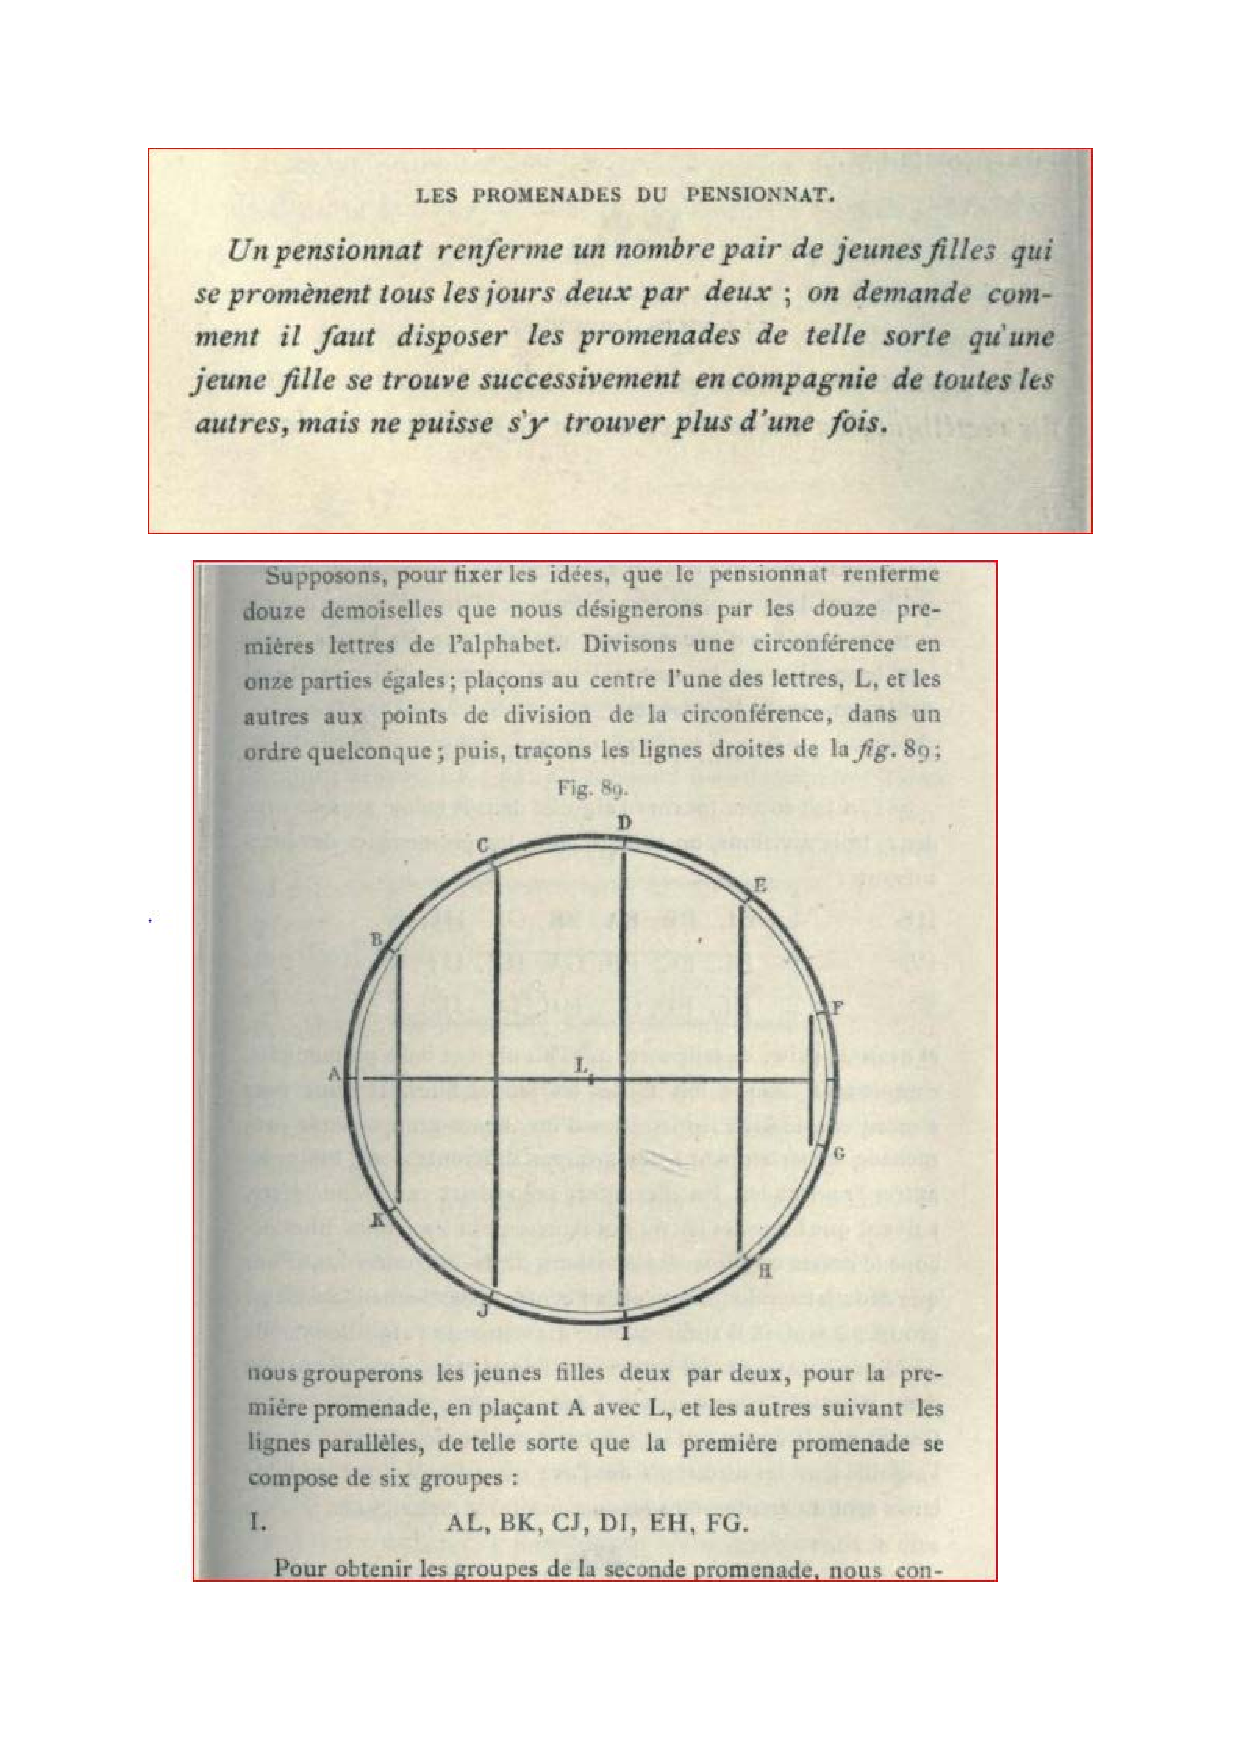
\includepdf[scale=.8, page=1, pagecommand=\section{Une approche mathématique}]{Projet_Tournois.pdf}
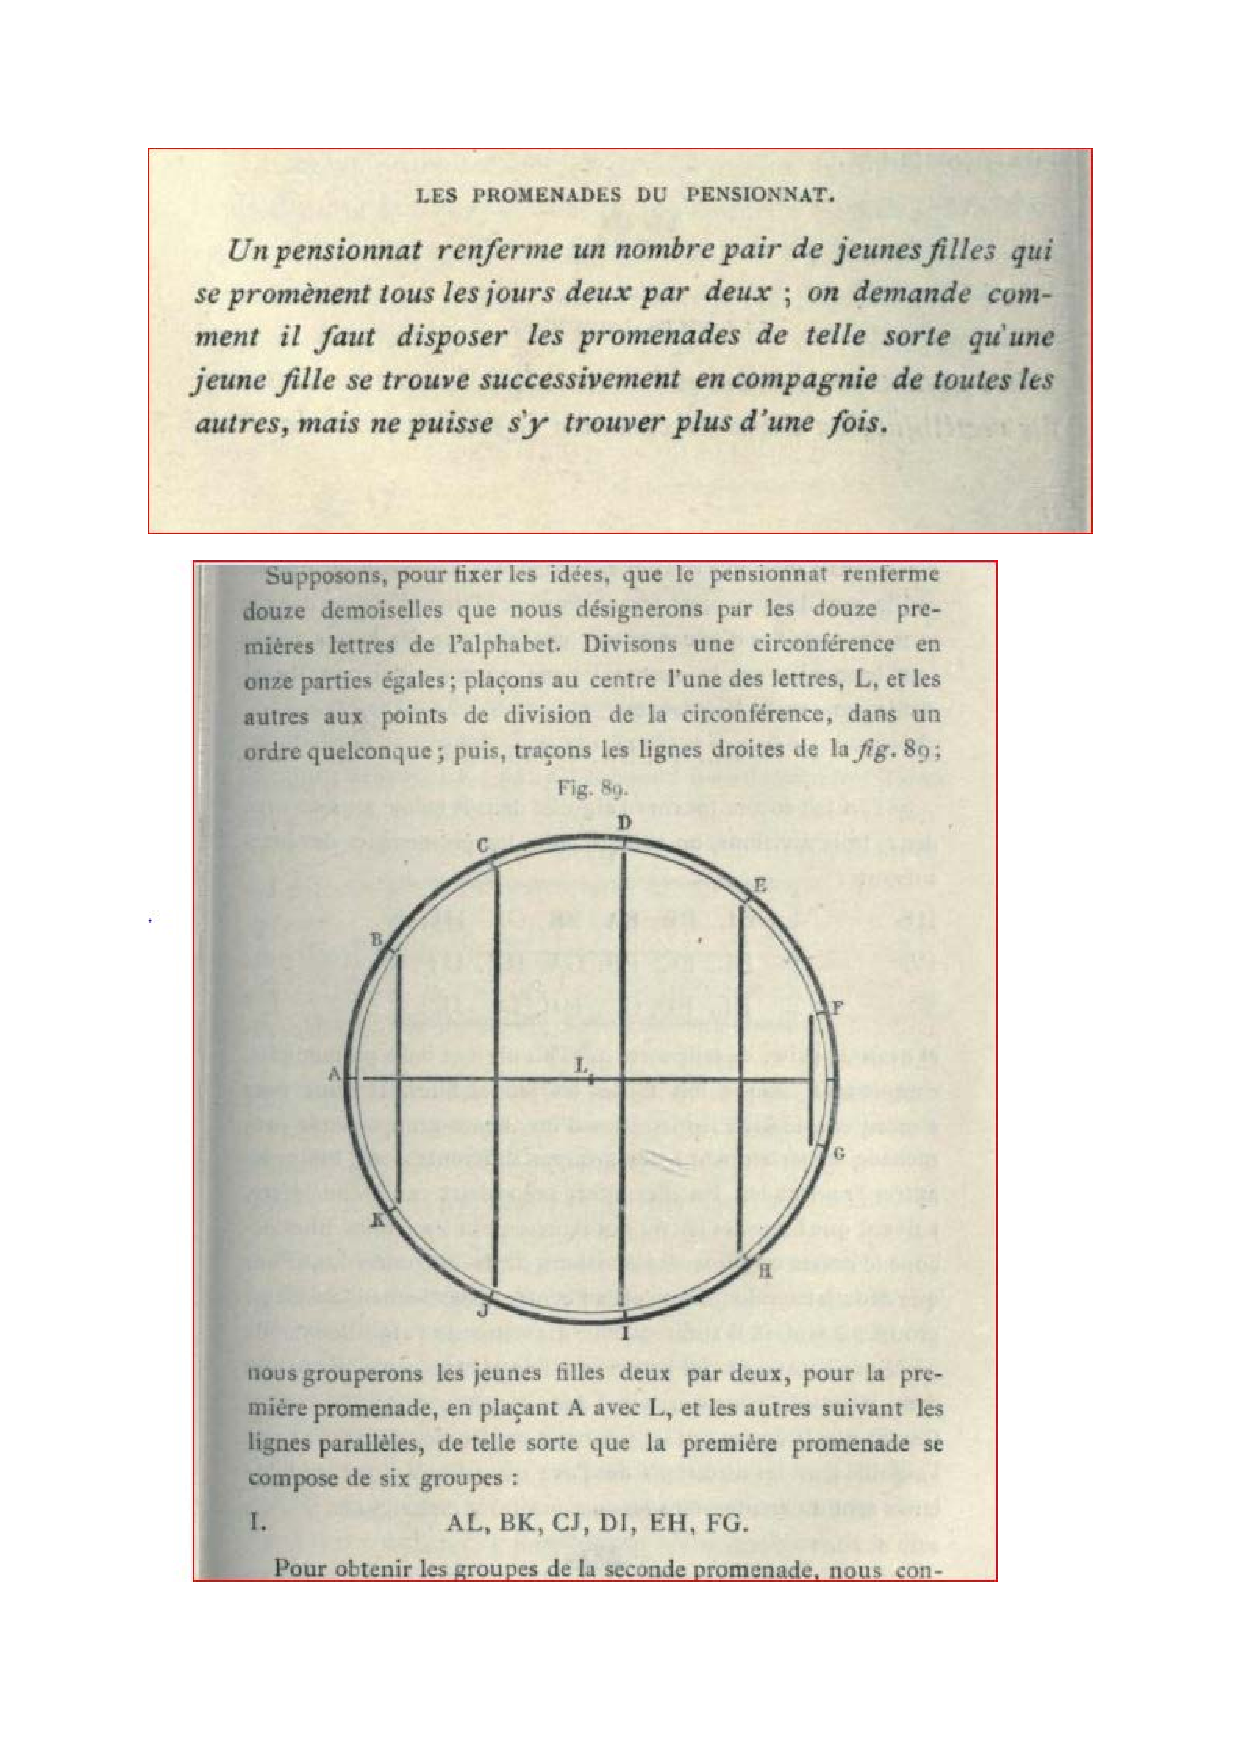
\includepdf[scale=.9, page=2-4]{Projet_Tournois.pdf}
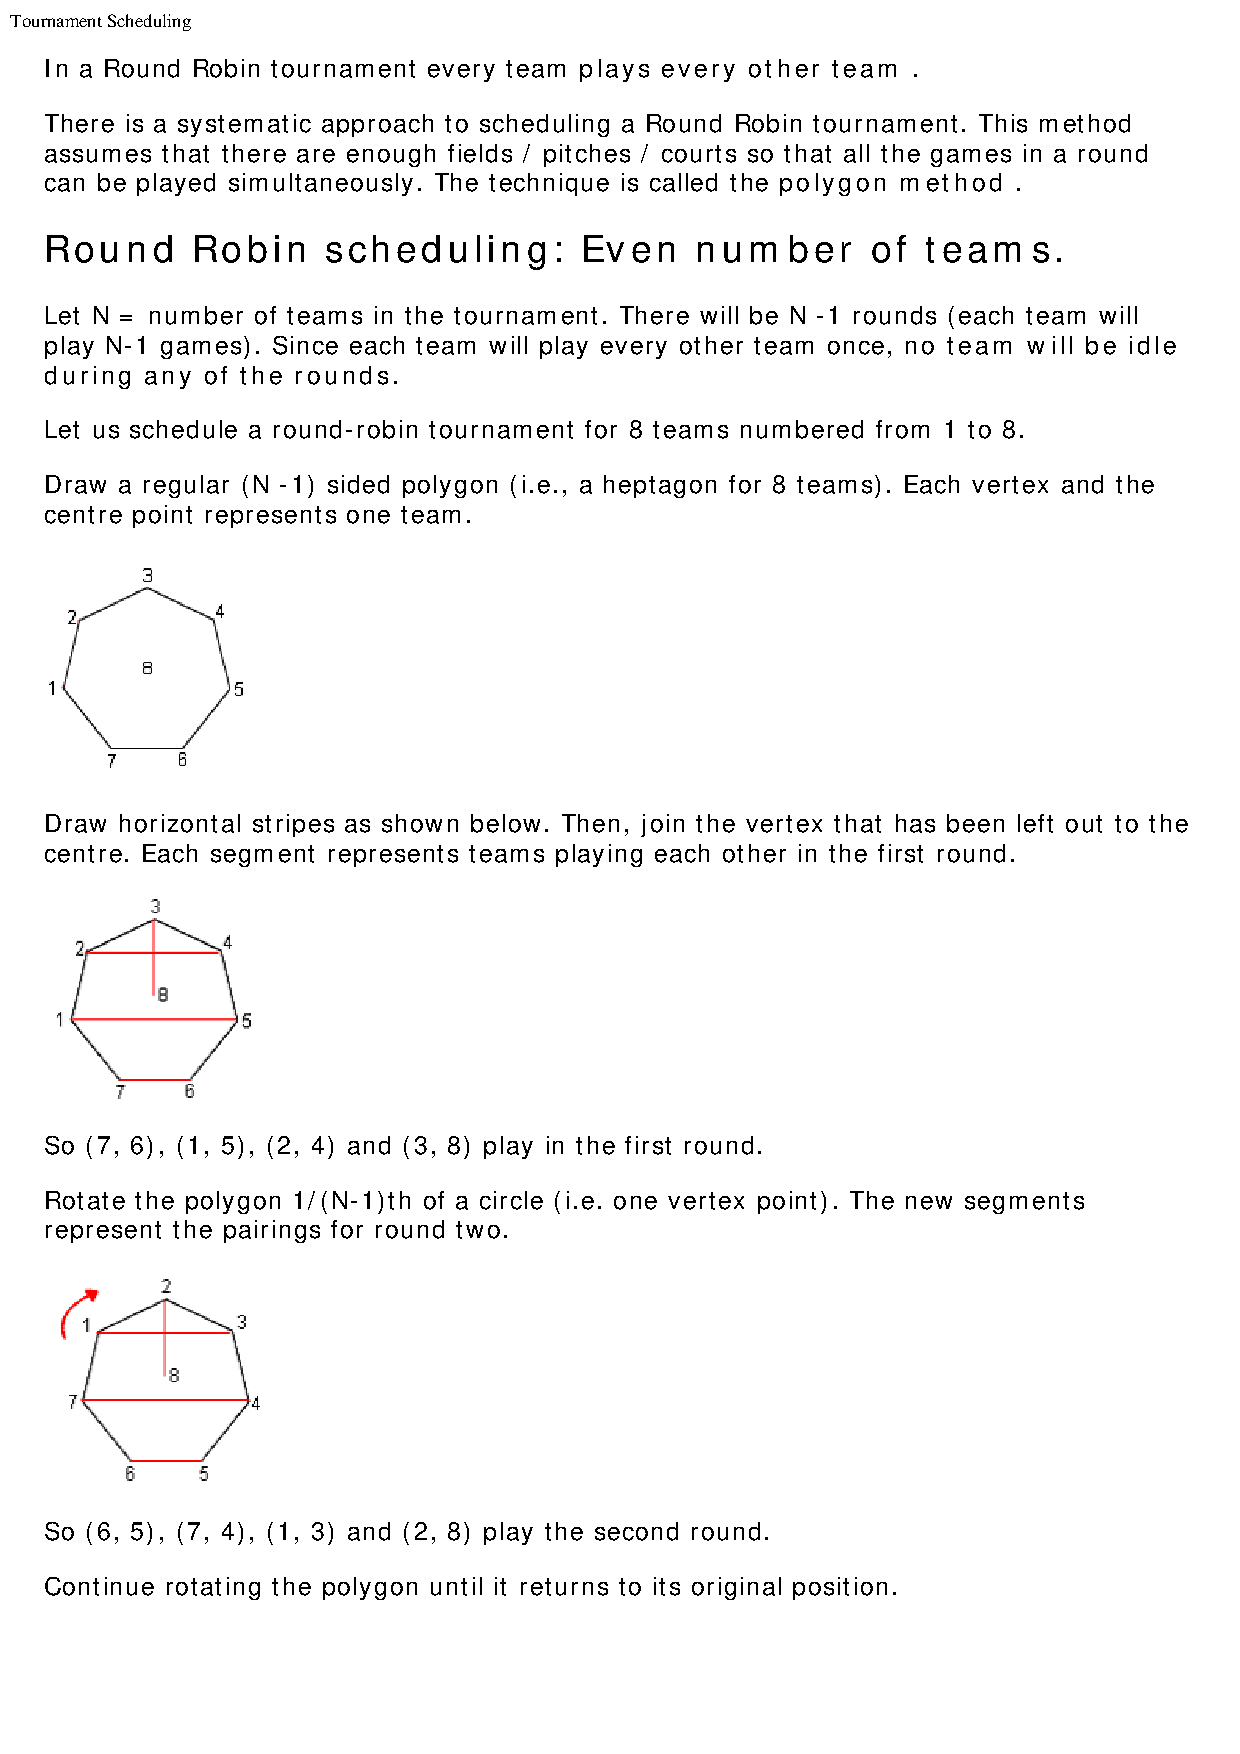
\includepdf[scale=.9, page=2-4]{Projet_Tournois_Bis.pdf}



\end{document}